%%%%%%%%%%%%%%%%%%%%%%%%%%%%%%%%%%%%%%%%%%%%%%%%%%%%%%%%%%%%%%%%%%%%%%%%%%%%%%%%
% ICMLA 2025/2026 — IEEE International Conference on Machine Learning and
% Applications
%
% Versão em Português (Brasil)
% Formato: IEEEtran (conference)
%%%%%%%%%%%%%%%%%%%%%%%%%%%%%%%%%%%%%%%%%%%%%%%%%%%%%%%%%%%%%%%%%%%%%%%%%%%%%%%%

\documentclass[conference]{IEEEtran}
\IEEEoverridecommandlockouts

\usepackage[utf8]{inputenc}
\usepackage[T1]{fontenc}
\usepackage{cite}
\usepackage{amsmath,amssymb,amsfonts}
\usepackage{algorithmic}
\usepackage{graphicx}
\usepackage{textcomp}
\usepackage{xcolor}
\usepackage{float}
\usepackage{multirow}
\usepackage{epstopdf}

\graphicspath{{../IJCNN/}{./}}

\def\BibTeX{{\rm B\kern-.05em{\sc i\kern-.025em b}\kern-.08em
    T\kern-.1667em\lower.7ex\hbox{E}\kern-.125emX}}

% -----------------------------------------------------------------------

\title{Recuperação de Imagens Orientada a Atributos por Fusão Adaptativa
       de Camadas com Mistura de Especialistas%
\thanks{Este trabalho foi financiado pelo Conselho Nacional de
        Desenvolvimento Científico e Tecnológico (CNPq, Brasil).}}

\author{%
\IEEEauthorblockN{Arlete T. Beuren, Vinícius C. Ribeiro,
                  Leonardo J. R. Pinto}
\IEEEauthorblockA{Universidade Tecnológica Federal do Paraná (UTFPR)\\
                  Santa Helena (PR), Brasil\\
                  \texttt{arletebeuren@utfpr.edu.br}}
\and
\IEEEauthorblockN{Jonathan de Matos}
\IEEEauthorblockA{Universidade Estadual de Ponta Grossa (UEPG)\\
                  Ponta Grossa (PR), Brasil\\
                  \texttt{jonathan@uepg.br}}
\and
\IEEEauthorblockN{Alceu S. Britto Jr.}
\IEEEauthorblockA{UEPG / Pontifícia Universidade Católica do Paraná
                  (PUCPR)\\
                  Brasil\\
                  \texttt{alceu@ppgia.pucpr.br}}
}

% -----------------------------------------------------------------------

\begin{document}

\maketitle

% -----------------------------------------------------------------------
\begin{abstract}

Este trabalho aborda o desafio de extrair eficazmente o conteúdo de
imagens com base em atributos visuais específicos — cor, textura ou sua
combinação — e propõe uma estratégia de fusão adaptativa baseada em
Mistura de Especialistas~(MoE).
Experimentos são conduzidos com cinco arquiteturas — ResNet-50, VGG-16,
iBOT, VMamba e LMFCN — sobre um conjunto de dados de moda contendo
1.000 imagens de cor e 1.000 imagens de textura.
O \emph{Experimento~1} confirma que camadas rasas são mais eficazes para
a classificação por cor, enquanto camadas profundas se destacam no
reconhecimento de textura — padrão consistentemente observado em todas as
arquiteturas avaliadas, das CNNs clássicas aos Transformers Visuais e
Modelos de Espaço de Estados.
O \emph{Experimento~2} demonstra que a concatenação simples de
características de camadas rasas e profundas geralmente não supera
representações especializadas de camada única.
O \emph{Experimento~3} introduz um modelo MoE treinável que, por meio
de um roteador aprendido, pondera adaptativamente as contribuições das
camadas rasa (sensível à cor) e profunda (sensível à textura) por imagem.
O MoE supera o Experimento~1 e o Experimento~2 em quase todas as
arquiteturas, atingindo até 98,00\% com VMamba em textura e 97,33\% com
iBOT em cor — melhorias de 2,24 e 1,46 pontos percentuais sobre as
melhores camadas individuais, respectivamente.

\end{abstract}

\begin{IEEEkeywords}
Redes Neurais Convolucionais, Modelos Profundos, Atributos Visuais,
Transformers Visuais, Modelos de Espaço de Estados, Mistura de
Especialistas, Recuperação de Imagens.
\end{IEEEkeywords}

% -----------------------------------------------------------------------
\section{Introdução}

Os avanços em redes neurais convolucionais (CNNs) têm viabilizado soluções
de visão computacional cada vez mais eficazes em aplicações industriais.
Um exemplo proeminente é a recuperação de imagens em comércio eletrônico,
onde consultas podem ser realizadas por texto, imagens ou combinações
multimodais~\cite{b1}.

Sistemas de Recuperação de Imagens Baseada em Conteúdo (CBIR) apresentam
desafios únicos e possuem aplicações além do comércio eletrônico, incluindo
imagens médicas, sistemas de informação geográfica e
vigilância~\cite{b12}.
Um desafio central reside na extração precisa de atributos visuais
relevantes, especialmente quando consultas são guiadas por propriedades
específicas como cor, textura ou sua combinação
(Fig.~\ref{fig_patterns}).

\begin{figure}[htbp]
\centerline{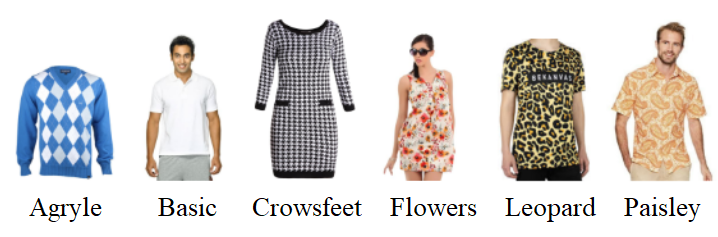
\includegraphics[width=0.48\textwidth]{fig_texture_samples.png}}
\caption{Seis padrões distintos baseados em cor e textura
         (adaptado de~\cite{b2}).}
\label{fig_patterns}
\end{figure}

A extração de características de cor e textura tem sido tema central em
CBIR.
Descritores clássicos de cor incluem histogramas e momentos de cor, que
capturam propriedades estatísticas como média, variância e assimetria das
distribuições cromáticas~\cite{b24}.
Para textura, métodos como filtros de Gabor e Padrões Binários Locais
(LBP) têm sido amplamente utilizados~\cite{b25}.

Com o advento do aprendizado profundo, Baloian et al.~\cite{b2}
demonstraram que diferentes camadas de CNNs exibem sensibilidade
específica a atributos, com camadas rasas sendo mais responsivas à
informação de cor e camadas profundas capturando padrões de textura.
Contudo, o comportamento de representações específicas por atributo em
arquiteturas modernas — Transformers Visuais e Modelos de Espaço de
Estados — permanece pouco explorado, e estratégias adaptativas de fusão
entre camadas especializadas ainda são escassas na literatura.

Neste trabalho, avaliamos e comparamos arquiteturas profundas clássicas e
modernas para classificação de imagens por cor e textura.
Analisamos representações por camada para investigar sua sensibilidade a
atributos visuais e a eficácia de diferentes estratégias de fusão.
Como contribuição principal, propõe-se um modelo de fusão adaptativa
baseado em Mistura de Especialistas~(MoE) que aprende, por imagem, os
pesos relativos das camadas rasa (cor) e profunda (textura) por meio de
um roteador treinável.

O conjunto de dados utilizado foi introduzido em~\cite{b2} e consiste em
imagens de moda incluindo chapéus, vestidos, camisas, meias, bolsas e
lenços, dividido em dois subconjuntos:
\begin{itemize}
  \item \textbf{Conjunto de cor}: 1.000 imagens em 10 classes de cor
        (vermelho, preto, azul, verde, amarelo, cinza, marrom, rosa,
        roxo e laranja), ilustradas na Fig.~\ref{fig_color_samples};
  \item \textbf{Conjunto de textura}: 1.000 imagens em 10 classes de
        padrão (xadrez, listrado, flores, leopardo, poás, básico, paisley,
        argyle, crowsfeet e paetê).
\end{itemize}

\begin{figure}[htbp]
\centerline{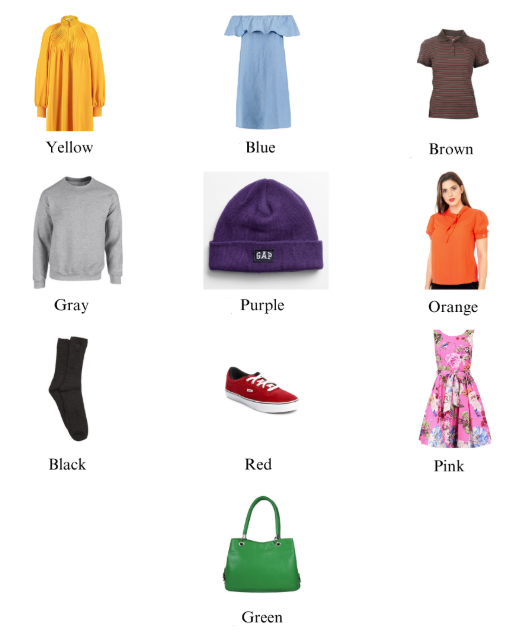
\includegraphics[width=0.48\textwidth]{fig_color_samples.png}}
\caption{Imagens de amostra de cada classe do conjunto de cor.}
\label{fig_color_samples}
\end{figure}

As principais contribuições deste trabalho são:
\begin{itemize}
  \item Uma análise abrangente da sensibilidade por camada a atributos
        visuais em CNNs clássicas, Transformers Visuais e Modelos de
        Espaço de Estados;
  \item Um benchmark comparativo de VGG-16, ResNet-50, iBOT, VMamba e
        LMFCN para classificação por cor e textura;
  \item Demonstração experimental de que a fusão por concatenação simples
        não melhora o desempenho em tarefas específicas por atributo;
  \item Proposta e avaliação de um modelo MoE que realiza fusão adaptativa
        de características de camadas rasa e profunda, superando
        concatenação e representações de camada única na maioria dos
        cenários.
\end{itemize}

Este artigo está organizado da seguinte forma.
A Seção~II revisa trabalhos relacionados.
A Seção~III descreve as arquiteturas backbone avaliadas.
A Seção~IV detalha a metodologia experimental.
A Seção~V apresenta os resultados.
A Seção~VI discute os achados e a Seção~VII conclui o artigo.

% -----------------------------------------------------------------------
\section{Trabalhos Relacionados}

O uso de redes neurais convolucionais para representar similaridade entre
objetos tem sido amplamente explorado.
Baloian et al.~\cite{b2} investigaram o comportamento das camadas da
ResNet-50 para recuperação por cor e textura, demonstrando que camadas
convolucionais rasas são mais sensíveis à cor, enquanto camadas profundas
capturam melhor padrões de textura.
Características foram extraídas da ResNet-50 pré-treinada no
ImageNet~\cite{b3} com Pooling Global por Média (GAP) em cada bloco
residual, e k-vizinhos mais próximos (kNN) foram usados para
classificação com 5 repetições de holdout estratificado 70/30.

A natureza hierárquica das representações em redes profundas foi
investigada desde o trabalho seminal de Zeiler e Fergus~\cite{bzeiler},
que demonstraram visualmente que camadas rasas de CNNs respondem a bordas
e cores, enquanto camadas profundas codificam padrões estruturais
complexos.
Análises análogas para Transformers Visuais foram conduzidas por
Kazami et al.~\cite{bkazami}, revelando que blocos iniciais de ViTs
preservam informação espacial de baixo nível enquanto blocos finais
capturam semântica global.
Em contraste com esses trabalhos, que realizam análises qualitativas ou
baseadas em visualização, o presente estudo conduz uma avaliação
quantitativa sistemática da sensibilidade por camada a atributos visuais
específicos (cor e textura), estende a análise à arquitetura VMamba
(Modelo de Espaço de Estados) ainda não coberta na literatura de análise
por camada, e propõe um mecanismo de fusão adaptativa treinável
fundamentado nessas descobertas.

Vários estudos exploram aprendizado de representações para reconhecimento
de objetos e atributos.
Liang et al.~\cite{b10} empregaram redes neurais para aprender
características discriminativas baseadas em categorias de objetos, enquanto
Gan et al.~\cite{b11} propuseram técnicas de generalização multi-domínio
para aprendizado de atributos entre domínios.
Arquiteturas siamesas foram investigadas para classificação refinada;
Moresco et al.~\cite{b8} demonstraram que combinar características de
camadas intermediárias melhora a classificação de espécies de plantas,
destacando a natureza complementar de representações multi-camada.

Descritores clássicos de textura e cor permanecem relevantes para sistemas
CBIR.
Irtaza et al.~\cite{b13} propuseram um framework de extração de textura
baseado em pacotes wavelet e autovalores de filtros de Gabor.
Lin et al.~\cite{b15} introduziram matrizes de co-ocorrência de cor (CCM),
diferença entre pixels de padrões de varredura (DBPSP) e agrupamento
baseado em histograma de cor (CHKM).

A fusão de características multi-camada foi proposta para combinar
representações de diferentes profundidades de rede.
As estratégias incluem fusão antecipada (concatenação de características),
fusão tardia (combinação no nível de decisão) e fusão aprendida usando
mecanismos de atenção~\cite{b26,b27}.
Contudo, a eficácia dessas abordagens para tarefas específicas por atributo
permanece insuficientemente estudada.

Avanços recentes têm desafiado o domínio dos modelos baseados em
Transformer.
A arquitetura Mamba~\cite{b16} é um Modelo de Espaço de Estados
Estruturado (SSM) com complexidade temporal linear, e o framework
iBOT~\cite{b17} introduziu modelagem mascarada de imagens com
tokenizador online para aprendizado de representações visuais
auto-supervisionado.
O framework LMFCN~\cite{b28} treina Redes Totalmente Convolucionais cujas
representações são otimizadas para classificação com SVM de grande margem.

A Mistura de Especialistas~(MoE) foi originalmente proposta por
Jacobs et al.~\cite{bmoe_orig} como uma arquitetura modular em que um
roteador aprende a dividir o espaço de entrada entre especialistas locais.
Trabalhos recentes exploram MoE para fusão multimodal de imagens: Cao
et al.~\cite{bmoe_cao} propuseram MoE-Fusion, combinando especialistas
locais e globais por meio de um roteador multimodal com porta para fusão
dinâmica de imagens.
Contudo, a aplicação de MoE para seleção adaptativa de camada por
profundidade dentro de um único backbone para atributos visuais específicos
permanece inexplorada.
Este trabalho preenche essa lacuna propondo um roteador treinável que
aprende, por imagem, quanto ponderar a representação da camada rasa
(cor) em relação à da camada profunda (textura).

% -----------------------------------------------------------------------
\section{Modelos Backbone Avaliados}

Esta seção descreve as cinco arquiteturas backbone utilizadas nos
experimentos.

\subsection{ResNet-50}

A ResNet-50~\cite{b4} é uma CNN de 50 camadas que emprega aprendizado
residual por meio de conexões de atalho baseadas em identidade, mitigando
a degradação do gradiente e possibilitando treinamento estável em grandes
profundidades.
No Experimento~1, características são extraídas de cada bloco residual
via GAP (dimensões: 256, 512, 1024 e 2048).
No modelo MoE, a camada rasa corresponde ao Bloco Residual~1~(256d) e a
camada profunda ao Bloco Residual~3~(1024d)
(Fig.~\ref{fig_resnet}).

\begin{figure}[htbp]
\centerline{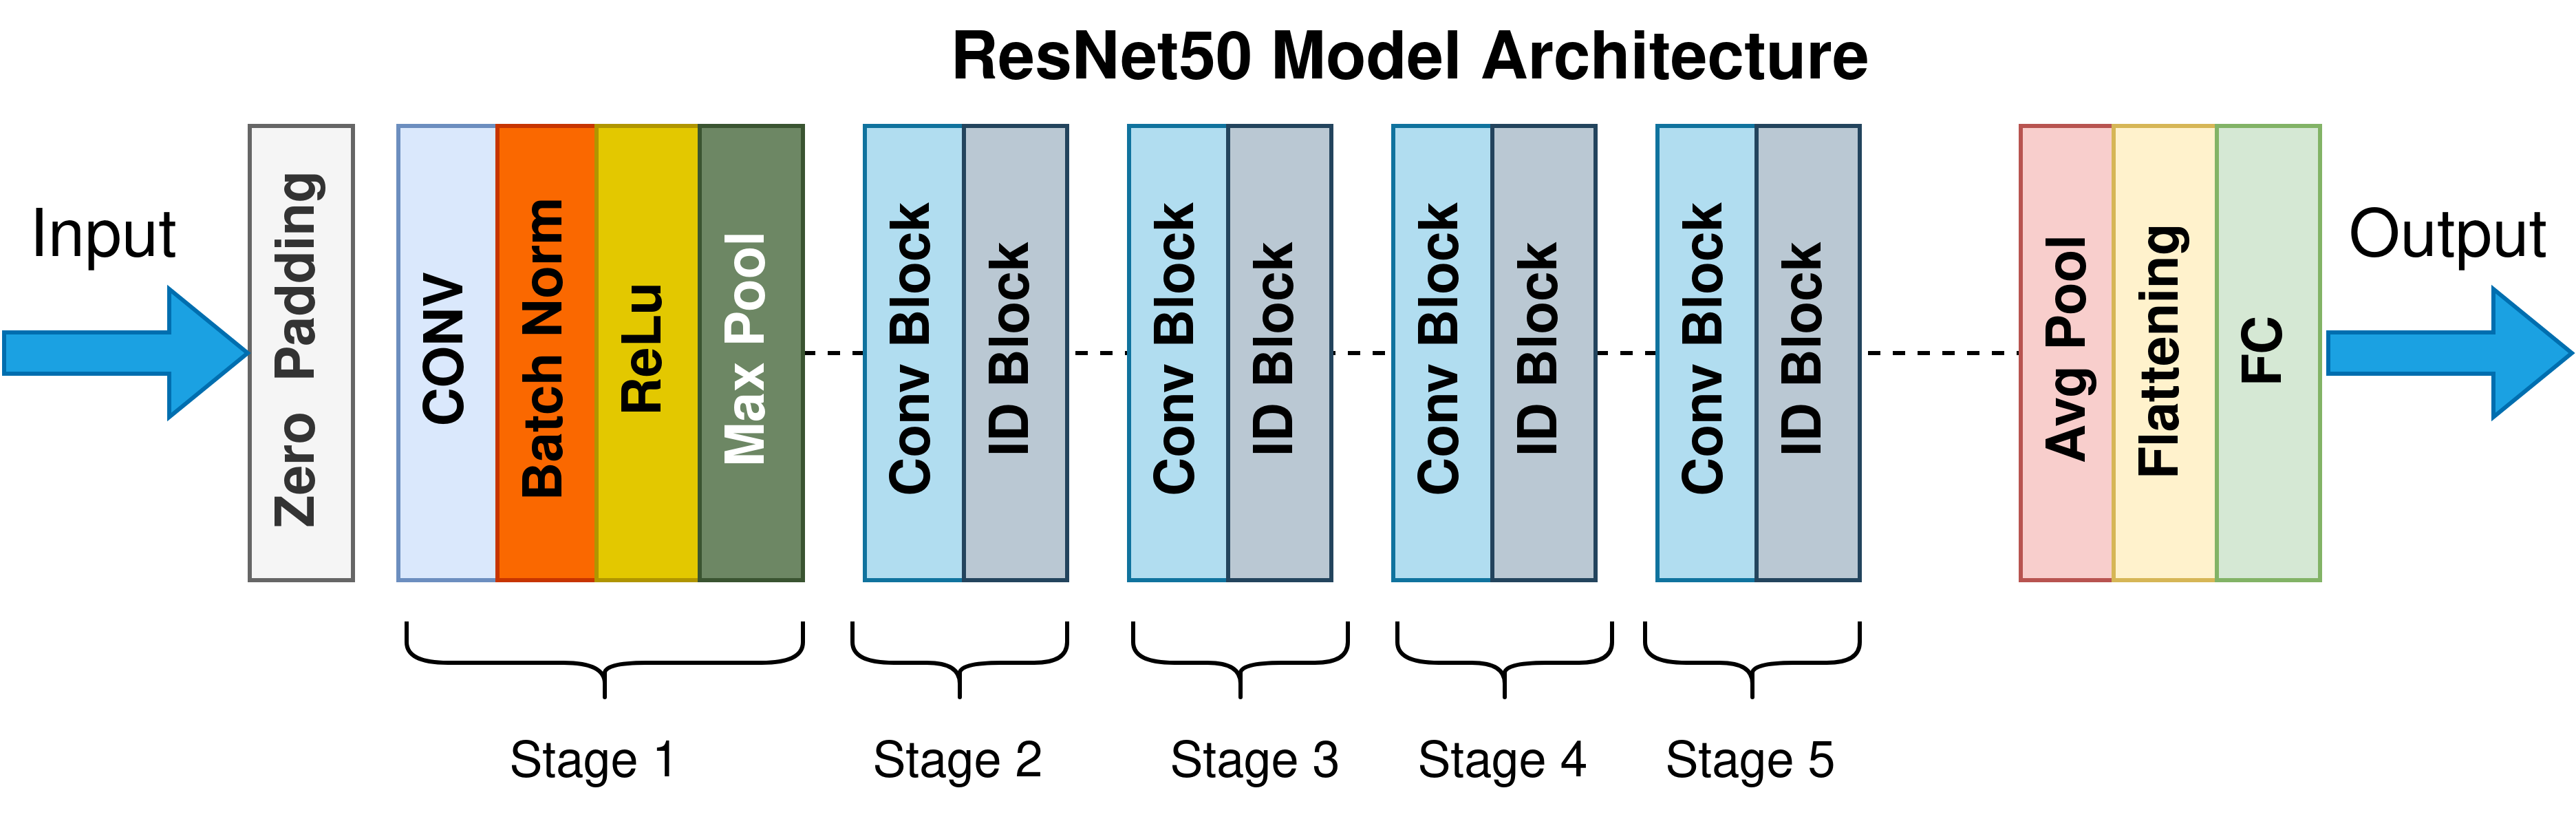
\includegraphics[width=0.48\textwidth]{resnet50.png}}
\caption{Arquitetura ResNet-50. Adaptado de Mukherjee~\cite{b23},
         baseado em He et al.~\cite{b4}.}
\label{fig_resnet}
\end{figure}

\subsection{VGG-16}

A VGG-16~\cite{b7} emprega uma arquitetura homogênea com camadas
convolucionais $3 \times 3$ empilhadas em 5 blocos convolucionais com
dimensões de saída 64, 128, 256, 512 e 512.
No modelo MoE, a camada rasa corresponde ao Bloco~1~(64d) e a camada
profunda ao Bloco~3~(256d) (Fig.~\ref{fig_vgg}).

\begin{figure}[htbp]
\centerline{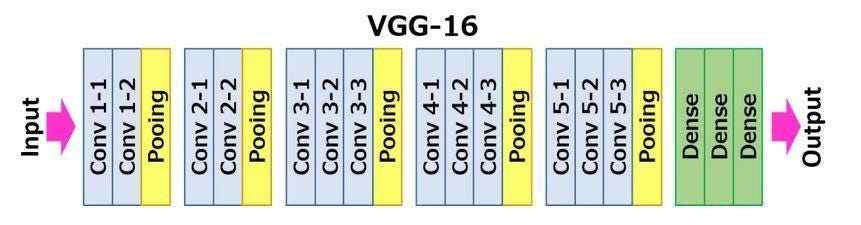
\includegraphics[width=0.48\textwidth]{VGG16.jpg}}
\caption{Arquitetura VGG-16.
         Fonte: Simonyan \& Zisserman~\cite{b7}.}
\label{fig_vgg}
\end{figure}

\subsection{VMamba}

A VMamba~\cite{b16} é um Modelo de Espaço de Estados Estruturado (SSM)
que processa sequências em tempo linear por meio de um mecanismo de
varredura seletiva.
Utilizamos a variante VMamba-Tiny; características são extraídas de cada
um de seus quatro estágios via GAP (dimensões: 96, 192, 384 e 768).
No MoE, a camada rasa é o Estágio~1~(192d) e a camada profunda é o
Estágio~2~(384d) (Fig.~\ref{fig_mamba}).

\begin{figure}[htbp]
\centerline{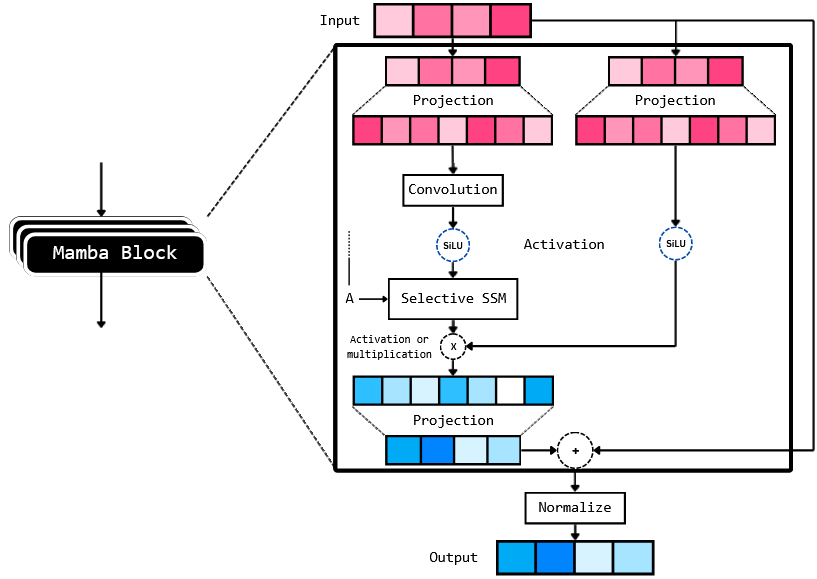
\includegraphics[width=0.48\textwidth]{Vmamba.png}}
\caption{Diagrama do bloco Mamba.
         Fonte: Gu \& Dao~\cite{b16}.}
\label{fig_mamba}
\end{figure}

\subsection{iBOT}

O iBOT~\cite{b17} é um framework auto-supervisionado baseado em
Transformers Visuais (ViT) com modelagem mascarada de imagens e
tokenizador online.
Utilizamos o backbone ViT-S/16; características são extraídas de cada
um de seus 12 blocos transformer via token CLS (384 dimensões cada).
No MoE, a camada rasa é o Bloco~2 e a camada profunda é o Bloco~9
(Fig.~\ref{fig_ibot}).

\begin{figure}[htbp]
\centerline{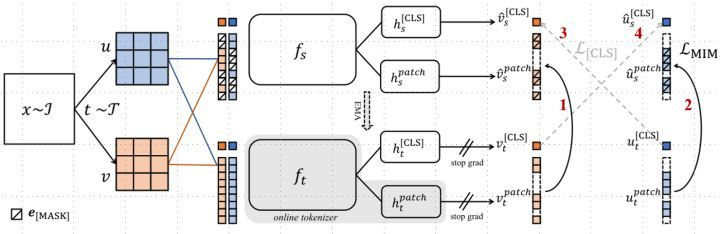
\includegraphics[width=0.48\textwidth]{Ibot.jpg}}
\caption{Visão geral do framework iBOT.
         Fonte: Zhou et al.~\cite{b17}.}
\label{fig_ibot}
\end{figure}

\subsection{LMFCN}

O framework LMFCN~\cite{b28} treina Redes Totalmente Convolucionais (FCNs)
cujas representações aprendidas são otimizadas para classificação SVM de
grande margem.
Avaliamos arquiteturas TCNN (3 a 6 camadas) treinadas do zero e variantes
da ResNet-18 pré-treinada com camadas finais removidas
(Fig.~\ref{fig_lmfcn}).
O LMFCN é incluído como arquitetura de referência apenas para análise de
comportamento por camada, sendo avaliado somente nos Experimentos~1 e~2,
uma vez que integrar um roteador MoE treinável ao seu framework exigiria
modificações arquiteturais não triviais.

\begin{figure}[htbp]
\centerline{\includegraphics[width=0.48\textwidth]{CNNSV4.eps}}
\caption{Visão geral do LMFCN.
         Fonte: de Matos et al.~\cite{b28}.}
\label{fig_lmfcn}
\end{figure}

% -----------------------------------------------------------------------
\section{Metodologia Experimental}

\subsection{Conjunto de Dados e Protocolo}

O conjunto de dados foi introduzido em~\cite{b2} e consiste em 10 classes
de cor e 10 classes de textura com 100 imagens por classe, totalizando
1.000 imagens por tarefa.
Os dados foram divididos em 70\% para treinamento e 30\% para teste em
5 repetições de holdout estratificado.
Seguindo o protocolo estabelecido em~\cite{b2} e amplamente adotado na
literatura CBIR baseada em atributos, os vetores de características são
avaliados com um classificador k-vizinhos mais próximos (kNN) ($k=5$,
distância Euclidiana).
Para a avaliação de recuperação, o conjunto de treinamento é utilizado
como galeria de busca, garantindo que os conjuntos de consulta e base de
dados sejam disjuntos e evitando correspondências triviais.

\subsection{Análise de Sensibilidade por Camada}

Para cada arquitetura, características são extraídas de cada camada ou
bloco de processamento individualmente.
CNNs utilizam GAP para produzir um único vetor de características por
camada; o iBOT utiliza o token CLS; o VMamba aplica GAP ao mapa de
características de cada estágio.
Para o LMFCN, avaliamos variantes TCNN (3–6 camadas) e ResNet-18 com
2 ou 4 blocos residuais.

\subsection{Fusão por Concatenação Camada Rasa--Profunda}

Para cada backbone, características da melhor camada de cor~(E) e da
melhor camada de textura~(D) são concatenadas:
$z = [f_E \; ; \; f_D]$, e o vetor resultante é avaliado com kNN.

\subsection{Fusão Adaptativa com Mistura de Especialistas}

O modelo MoE proposto aprende, por imagem, pesos adaptativos $\alpha$ e
$\beta$ para as camadas rasa e profunda, respectivamente.

\textbf{Arquitetura.} Para cada backbone, duas cabeças de projeção $h_E$
e $h_D$ — cada uma composta por uma camada linear, LayerNorm e ReLU —
mapeiam características de dimensões heterogêneas para um espaço comum
de dimensão $d=256$.
Um Roteador (MLP de duas camadas com Softmax) recebe a concatenação
$[h_E(f_E) \; ; \; h_D(f_D)]$ e produz pesos $\alpha$ e $\beta$ com
$\alpha + \beta = 1$.
O embedding final é:
\begin{equation}
    z = \alpha \cdot h_E(f_E) + \beta \cdot h_D(f_D).
    \label{eq:moe}
\end{equation}

O backbone é congelado durante o treinamento; apenas $h_E$, $h_D$ e o
Roteador são atualizados.
Uma cabeça linear auxiliar supervisiona o treinamento com perda de
entropia cruzada; na avaliação, apenas os embeddings $z$ são utilizados
com kNN.

\textbf{Protocolo de treinamento.}
Otimizador AdamW, $lr = 10^{-4}$, decaimento de pesos $= 10^{-5}$,
CosineAnnealingLR com $T_{\max} = 30$ épocas, tamanho de lote 32,
aumento de dados básico (recorte aleatório 224$\times$224 e espelhamento
horizontal) apenas durante o treinamento.
Avaliação final: kNN com $k=5$ e StandardScaler nos embeddings $z$, sob
o mesmo protocolo de holdout com 5 repetições.

A Tabela~\ref{tab_moe_config} resume as configurações de camada rasa e
profunda por backbone no modelo MoE.

\begin{table}[htbp]
\caption{Configuração de camada rasa e profunda por backbone no MoE.}
\begin{center}
\begin{tabular}{c|c|c|c|c}
\hline
\textbf{Backbone} & \textbf{Rasa (E)} & \textbf{Dim~E}
                  & \textbf{Profunda (D)} & \textbf{Dim~D} \\
\hline
VGG-16    & Bloco 1       & 64   & Bloco 3       & 256  \\
ResNet-50 & Bl. Res. 1    & 256  & Bl. Res. 3    & 1024 \\
iBOT      & Bloco 2       & 384  & Bloco 9       & 384  \\
VMamba    & Estágio 1     & 192  & Estágio 2     & 384  \\
\hline
\end{tabular}
\label{tab_moe_config}
\end{center}
\end{table}

% -----------------------------------------------------------------------
\section{Resultados Experimentais}

Os resultados estão organizados em duas partes.
A primeira~(Seções~V-A e~V-B) analisa o comportamento por camada dos
embeddings de cada backbone em relação à cor e textura, usando a acurácia
kNN como proxy para discriminabilidade do embedding.
O objetivo aqui não é otimizar a classificação, mas caracterizar quais
camadas melhor capturam cada atributo visual.
A segunda parte~(Seções~V-C a~V-E) avalia estratégias de fusão e, por
fim, os mesmos embeddings sob protocolo CBIR com mAP@10, R@1 e R@5.

\subsection{Sensibilidade por Camada}

A Tabela~\ref{tab_best_layer} resume a melhor camada por backbone para
classificação por cor e textura.
Em todas as arquiteturas, camadas rasas consistentemente atingem maior
acurácia de cor, enquanto camadas profundas são mais eficazes para textura
— confirmando e estendendo o padrão originalmente reportado para a
ResNet-50 em~\cite{b2}.
Na VGG-16, a Camada~1 atinge 95,13\% para cor, enquanto a Camada~4
alcança 94,73\% para textura.
A ResNet-50 segue a mesma tendência: Bloco Residual~2 para cor~(95,87\%)
e Bloco~3 para textura~(93,27\%).
O iBOT exibe o gradiente mais acentuado entre seus 12 blocos transformer
— a acurácia de cor cai de 94,53\% no Bloco~0 para 62,80\% no Bloco~11,
enquanto a textura sobe para 97,20\% no Bloco~9, o maior valor entre
todas as arquiteturas avaliadas.
O VMamba exibe uma versão mais comprimida do mesmo padrão em seus quatro
estágios, com o Estágio~1 sendo o melhor para cor~(94,41\%) e o
Estágio~2 para textura~(95,76\%).

\begin{table}[htbp]
\caption{Melhor camada por backbone para classificação por cor e textura
         (\%). Negrito: maior valor por coluna de atributo.}
\begin{center}
\begin{tabular}{c|c|c|c|c|c|c}
\hline
\textbf{Backbone} & \textbf{Melhor Cor} & \textbf{Cor} & \textbf{Dp}
                  & \textbf{Melhor Tex.} & \textbf{Tex.} & \textbf{Dp} \\
\hline
VGG-16    & Camada 1 & 95,13          & 0,81 & Camada 4 & 94,73          & 0,74 \\
ResNet-50 & BR 2     & \textbf{95,87} & 0,50 & BR 3     & 93,27          & 0,25 \\
iBOT      & Bloco 2  & \textbf{95,87} & 1,05 & Bloco 9  & \textbf{97,20} & 0,54 \\
VMamba    & Est.\ 1  & 94,41          & 0,52 & Est.\ 2  & 95,76          & 0,84 \\
\hline
\end{tabular}
\label{tab_best_layer}
\end{center}
\end{table}

A Fig.~\ref{fig_depth} ilustra as curvas completas de acurácia por
profundidade, exibindo o padrão inverso entre cor e textura em cada
backbone.

\begin{figure}[htbp]
\centerline{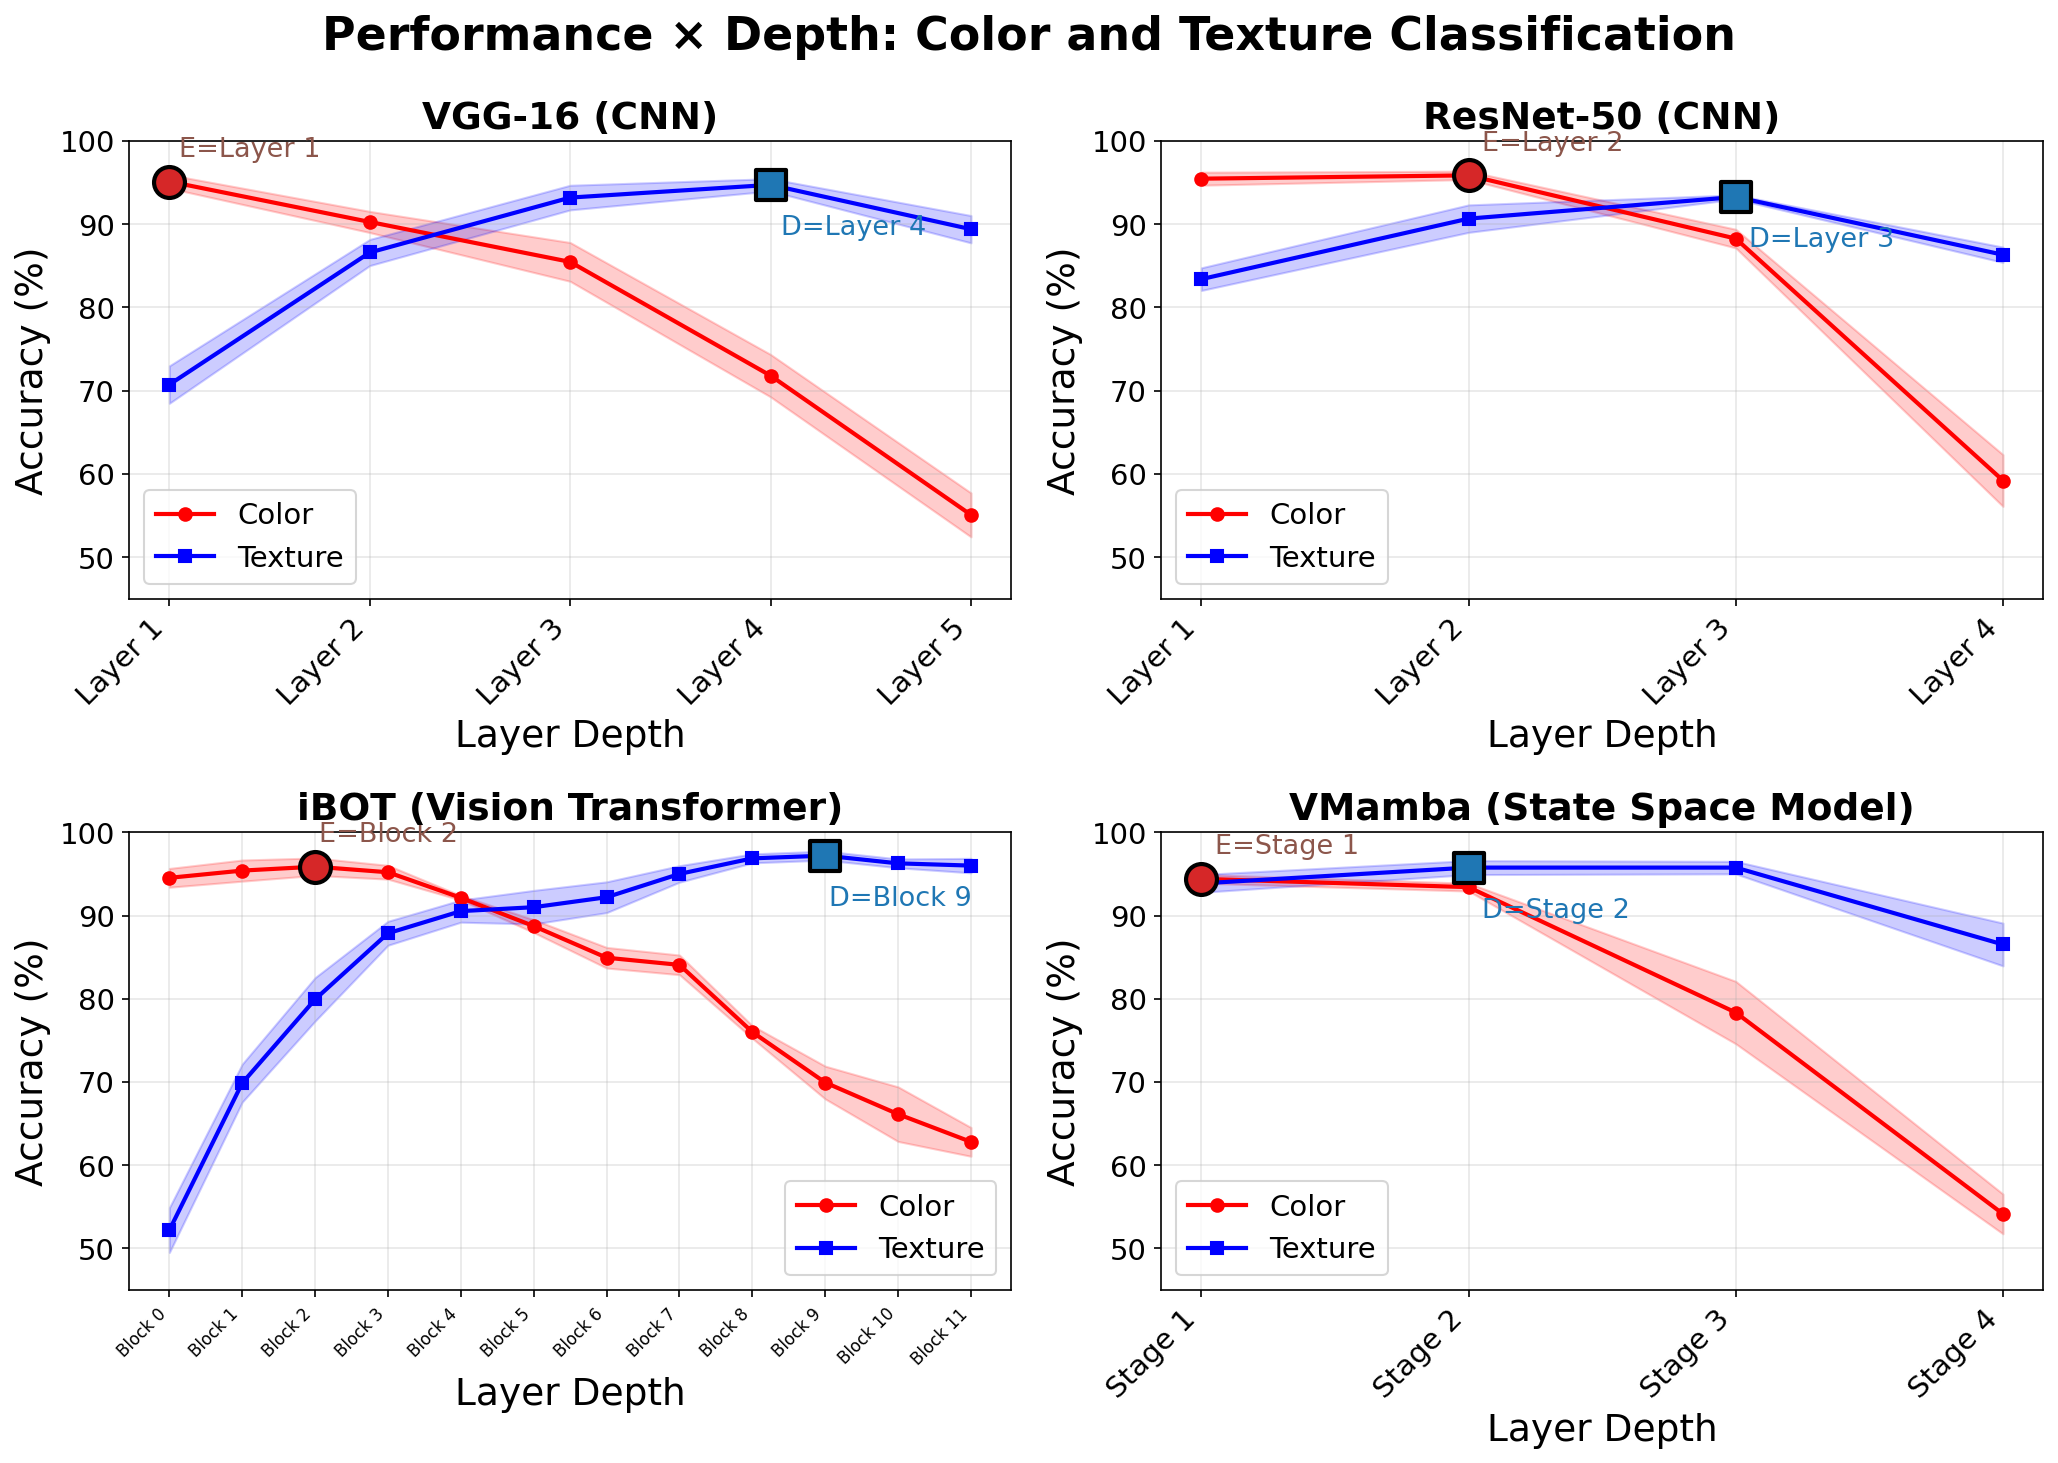
\includegraphics[width=0.48\textwidth]{curvas_desempenho_profundidade.png}}
\caption{Desempenho por profundidade: classificação por cor e textura
         para VGG-16, ResNet-50, iBOT e VMamba. Marcadores indicam a
         melhor camada por atributo (E=cor, D=textura).}
\label{fig_depth}
\end{figure}

\subsection{Sensibilidade por Camada --- LMFCN}

A Tabela~\ref{tab1} apresenta os resultados do LMFCN.
No conjunto de textura, o aumento de profundidade do TCNN melhora
consistentemente o desempenho.
No conjunto de cor, maior acurácia é obtida em camadas mais rasas.
O LMFCN com seu classificador SVM atingiu 96,87\%$\pm$0,9 em textura
(ResNet-18 com 2 blocos) e 97,73\%$\pm$0,95 em cor (TCNN3).

\begin{table}[htbp]
\caption{Acurácia dos blocos convolucionais (BC) e blocos residuais (BR)
         da ResNet-18 e camadas TCNN usando LMFCN.}
\begin{center}
\begin{tabular}{c|c|c|c|c|c}
\hline
\textbf{Método} & \textbf{Cor} & \textbf{Dp}
                & \textbf{Tex.} & \textbf{Dp} & \textbf{Dim} \\
\hline
TCNN3 Camada 3      & \textbf{95,94} & 0,43 & \textbf{58,27} & 1,30 & 640  \\
TCNN4 Camada 4      & \textbf{94,80} & 0,65 & \textbf{60,40} & 2,60 & 640  \\
TCNN5 Camada 5      & 95,40 & 0,96 & \textbf{62,93} & 1,65 & 640  \\
TCNN6 Camada 6      & 94,53 & 0,84 & \textbf{64,34} & 2,69 & 640  \\
ResNet-18(2) BR1    & \textbf{96,13} & 0,73 & 84,87 & 1,38 & 640  \\
ResNet-18(2) BR2    & 91,93 & 0,98 & \textbf{91,00} & 1,62 & 1280 \\
ResNet-18(4) BR1    & \textbf{95,93} & 0,98 & 84,13 & 1,59 & 640  \\
ResNet-18(4) BR3    & 89,53 & 1,37 & \textbf{92,47} & 1,48 & 2560 \\
\hline
\end{tabular}
\label{tab1}
\end{center}
\end{table}

\subsection{Resultados da Fusão por Concatenação Rasa--Profunda}

A Tabela~\ref{tab5} mostra a configuração de fusão por backbone, e as
Tabelas~\ref{tab6} e~\ref{tab7} apresentam os resultados.

\begin{table}[htbp]
\caption{Configuração de fusão por backbone.}
\begin{center}
\begin{tabular}{c|c|c|c|c|c}
\hline
\textbf{Backbone} & \textbf{E (cor)} & \textbf{Dim E}
                  & \textbf{D (tex.)} & \textbf{Dim D} & \textbf{Dim z} \\
\hline
VGG-16    & Cam. 1  & 64  & Cam. 4  & 512  & 576  \\
ResNet-50 & BR 2    & 512 & BR 3    & 1024 & 1536 \\
iBOT      & Bl.\ 2  & 384 & Bl.\ 9  & 384  & 768  \\
VMamba    & Est.\ 1 & 96  & Est.\ 2 & 192  & 288  \\
\hline
\end{tabular}
\label{tab5}
\end{center}
\end{table}

\begin{table}[htbp]
\caption{Resultados da fusão por concatenação para classificação por cor.}
\begin{center}
\begin{tabular}{c|c|c|c|c}
\hline
\textbf{Backbone} & \textbf{E (cor)} & \textbf{D (tex.)}
                  & \textbf{Z (fusão)} & \textbf{$\Delta$} \\
\hline
VGG-16    & \textbf{95,13\%} & 71,80\% & 86,13\% & $-$9,00\%  \\
ResNet-50 & \textbf{95,87\%} & 88,27\% & 94,13\% & $-$1,73\%  \\
iBOT      & \textbf{96,93\%} & 81,33\% & 85,13\% & $-$11,80\% \\
VMamba    & \textbf{94,80\%} & 93,93\% & 94,13\% & $-$0,67\%  \\
\hline
\end{tabular}
\label{tab6}
\end{center}
\end{table}

\begin{table}[htbp]
\caption{Resultados da fusão por concatenação para classificação por
         textura.}
\begin{center}
\begin{tabular}{c|c|c|c|c}
\hline
\textbf{Backbone} & \textbf{E (cor)} & \textbf{D (tex.)}
                  & \textbf{Z (fusão)} & \textbf{$\Delta$} \\
\hline
VGG-16    & 70,73\% & \textbf{94,73\%} & 94,73\% & $+$0,00\% \\
ResNet-50 & 90,67\% & 93,27\%          & \textbf{93,53\%} & $+$0,27\% \\
iBOT      & 78,33\% & \textbf{87,80\%} & 88,07\% & $+$0,27\% \\
VMamba    & 88,40\% & \textbf{94,33\%} & 93,40\% & $-$0,93\% \\
\hline
\end{tabular}
\label{tab7}
\end{center}
\end{table}

Os resultados de fusão mostram que a concatenação simples geralmente não
melhora o desempenho de classificação.
Para cor, a fusão degradou consistentemente a acurácia em relação ao uso
isolado da camada especializada~(E), com o iBOT apresentando a maior
degradação~($-$11,80\%).
Para textura, os resultados foram mistos, com melhoras mínimas para
ResNet-50 e iBOT~($+$0,27\%) e degradação para VMamba~($-$0,93\%).

\subsection{Resultados da Fusão MoE Adaptativa}

A Tabela~\ref{tab_moe} apresenta os resultados do modelo MoE proposto.
Em comparação à extração de camada única e à fusão por concatenação, o
MoE supera ambos em quase todas as combinações backbone–atributo.

\begin{table}[htbp]
\caption{Resultados do modelo MoE para classificação por cor e textura.}
\begin{center}
\begin{tabular}{c|c|c|c|c}
\hline
\textbf{Backbone} & \textbf{MoE Cor (\%)} & \textbf{Dp}
                  & \textbf{MoE Tex. (\%)} & \textbf{Dp} \\
\hline
VGG-16    & 93,40 & 0,71 & 96,13 & 1,00 \\
ResNet-50 & 97,27 & 0,71 & \textbf{97,67} & 0,47 \\
iBOT      & \textbf{97,33} & 0,56 & 95,47 & 0,96 \\
VMamba    & 96,93 & 1,02 & \textbf{98,00} & 0,73 \\
\hline
\end{tabular}
\label{tab_moe}
\end{center}
\end{table}

A Tabela~\ref{tab_comparacao} consolida a comparação entre as três
estratégias.

\begin{table}[htbp]
\caption{Comparação entre camada única (Exp.\,1), concatenação (Exp.\,2)
         e MoE (Exp.\,3). Valores em \%. $\Delta_1$: ganho sobre camada
         única; $\Delta_2$: ganho sobre concatenação.}
\begin{center}
\begin{tabular}{c|c|c|c|c|c|c}
\hline
\textbf{Config.} & \textbf{Exp.1} & \textbf{Exp.2}
                 & \textbf{MoE} & \textbf{$\Delta_1$}
                 & \textbf{$\Delta_2$} & \textbf{Melhor} \\
\hline
VGG Cor     & 95,13 & 86,13 & 93,40 & $-$1,73 & $+$7,27  & Exp.1 \\
VGG Tex.    & 94,73 & 94,73 & 96,13 & $+$1,40 & $+$1,40  & \textbf{MoE} \\
ResNet Cor. & 95,87 & 94,13 & 97,27 & $+$1,40 & $+$3,13  & \textbf{MoE} \\
ResNet Tex. & 93,27 & 93,53 & 97,67 & $+$4,40 & $+$4,13  & \textbf{MoE} \\
iBOT Cor    & 95,87 & 85,13 & 97,33 & $+$1,46 & $+$12,20 & \textbf{MoE} \\
iBOT Tex.   & 97,20 & 88,07 & 95,47 & $-$1,73 & $+$7,40  & Exp.1 \\
VMamba Cor. & 94,41 & 94,13 & 96,93 & $+$2,52 & $+$2,80  & \textbf{MoE} \\
VMamba Tex. & 95,76 & 93,40 & 98,00 & $+$2,24 & $+$4,60  & \textbf{MoE} \\
\hline
\end{tabular}
\label{tab_comparacao}
\end{center}
\end{table}

O MoE é o melhor método em 6 das 8 configurações avaliadas.
As duas exceções — VGG-16 cor e iBOT textura — correspondem a casos onde
uma única camada especializada já atinge desempenho muito elevado
(95,13\% e 97,20\%, respectivamente), deixando pouco espaço para melhora.
Notavelmente, o ganho do MoE sobre a concatenação é expressivo em todas
as configurações, particularmente para iBOT cor~($+$12,20~pp) e
VMamba textura~($+$4,60~pp).

\subsection{Avaliação CBIR: mAP@10, R@1 e R@5}

As Tabelas~\ref{tab_cbir_color} e~\ref{tab_cbir_texture} reportam a
avaliação de recuperação de cada embedding sob protocolo CBIR padrão.
Para cada imagem de teste usada como consulta, todas as imagens de
treinamento na galeria são ordenadas por distância Euclidiana; as métricas
são calculadas sobre os $K\!=\!10$ vizinhos mais próximos.
mAP@10 é a precisão média sobre os 10 itens mais próximos recuperados;
R@1 e R@5 indicam, respectivamente, a fração de consultas para as quais
a classe correta aparece no rank~1 e nos 5 primeiros.

\begin{table}[htbp]
\caption{Avaliação CBIR --- Cor (\%). Melhor valor por backbone em
         \textbf{negrito}.}
\begin{center}
\begin{tabular}{c|l|c|c|c}
\hline
\textbf{Backbone} & \textbf{Método} & \textbf{mAP@10}
                  & \textbf{R@1} & \textbf{R@5} \\
\hline
\multirow{4}{*}{VGG-16}
  & Camada rasa (E)          & \textbf{94,47} & \textbf{95,47} & \textbf{99,13} \\
  & Camada profunda (D)      & 72,92 & 72,20 & 91,53 \\
  & Concatenação             & 83,89 & 86,53 & 96,73 \\
  & MoE                      & 93,71 & 94,93 & 98,07 \\
\hline
\multirow{4}{*}{ResNet-50}
  & Camada rasa (E)          & 94,51 & 96,13 & 99,00 \\
  & Camada profunda (D)      & 86,25 & 87,67 & 97,20 \\
  & Concatenação             & 92,40 & 93,93 & 98,33 \\
  & MoE                      & \textbf{96,09} & \textbf{96,07} & \textbf{98,67} \\
\hline
\multirow{4}{*}{iBOT}
  & Camada rasa (E)          & 94,93 & 95,40 & 99,13 \\
  & Camada profunda (D)      & 71,85 & 72,00 & 92,47 \\
  & Concatenação             & 75,06 & 76,67 & 94,13 \\
  & MoE                      & \textbf{97,96} & \textbf{98,27} & \textbf{99,47} \\
\hline
\multirow{4}{*}{VMamba}
  & Camada rasa (E)          & 93,20 & 94,33 & 98,47 \\
  & Camada profunda (D)      & 91,73 & 93,13 & 98,33 \\
  & Concatenação             & 92,51 & 93,67 & 98,40 \\
  & MoE                      & \textbf{96,91} & \textbf{96,87} & \textbf{99,07} \\
\hline
\end{tabular}
\label{tab_cbir_color}
\end{center}
\end{table}

\begin{table}[htbp]
\caption{Avaliação CBIR --- Textura (\%). Melhor valor por backbone em
         \textbf{negrito}.}
\begin{center}
\begin{tabular}{c|l|c|c|c}
\hline
\textbf{Backbone} & \textbf{Método} & \textbf{mAP@10}
                  & \textbf{R@1} & \textbf{R@5} \\
\hline
\multirow{4}{*}{VGG-16}
  & Camada rasa (E)          & 70,87 & 70,33 & 91,27 \\
  & Camada profunda (D)      & 94,78 & 96,20 & \textbf{99,47} \\
  & Concatenação             & 94,53 & 96,13 & 99,27 \\
  & MoE                      & \textbf{95,98} & \textbf{96,80} & 99,07 \\
\hline
\multirow{4}{*}{ResNet-50}
  & Camada rasa (E)          & 90,35 & 90,80 & 99,07 \\
  & Camada profunda (D)      & 93,72 & 95,60 & 99,20 \\
  & Concatenação             & 93,05 & 94,47 & 98,87 \\
  & MoE                      & \textbf{97,88} & \textbf{98,13} & \textbf{99,20} \\
\hline
\multirow{4}{*}{iBOT}
  & Camada rasa (E)          & 78,90 & 79,33 & 94,33 \\
  & Camada profunda (D)      & \textbf{96,40} & \textbf{97,73} & \textbf{99,80} \\
  & Concatenação             & 96,30 & 97,67 & 99,73 \\
  & MoE                      & 95,10 & 95,40 & 98,53 \\
\hline
\multirow{4}{*}{VMamba}
  & Camada rasa (E)          & 87,66 & 88,80 & 97,33 \\
  & Camada profunda (D)      & 93,52 & 95,53 & 99,13 \\
  & Concatenação             & 93,05 & 95,07 & 99,13 \\
  & MoE                      & \textbf{97,89} & \textbf{98,27} & \textbf{99,33} \\
\hline
\end{tabular}
\label{tab_cbir_texture}
\end{center}
\end{table}

O MoE alcança as melhores métricas CBIR em 3 dos 4 backbones para cor
e 3 dos 4 para textura.
A exceção para iBOT textura espelha o resultado de acurácia: o Bloco~9
produz representações de textura tão discriminativas~(mAP@10 = 96,40\%)
que o roteador não consegue superá-las.
O ganho do MoE sobre a concatenação é particularmente expressivo para
iBOT cor~($+$22,90~pp em mAP@10), confirmando que a fusão adaptativa
resolve a degradação observada no Experimento~2.

% -----------------------------------------------------------------------
\section{Discussão}

Os resultados experimentais confirmam que o padrão de sensibilidade por
camada anteriormente observado em CNNs clássicas é consistentemente
observado em todas as arquiteturas avaliadas, incluindo Transformers
Visuais e Modelos de Espaço de Estados.
Em todos os backbones avaliados, camadas rasas capturam consistentemente
características mais adequadas para classificação por cor, enquanto
camadas profundas são mais eficazes para reconhecimento de textura —
coerente com os achados fundamentais de Zeiler e Fergus~\cite{bzeiler}
para CNNs e com as análises de ViT de Kazami et al.~\cite{bkazami}.
Este trabalho estende esses achados quantitativamente para tarefas de
classificação específicas por atributo e ao VMamba, uma arquitetura de
Modelo de Espaço de Estados ainda não coberta na literatura de análise
por camada.

A acurácia excepcional do iBOT em textura~(97,20\%) sugere que o
objetivo de modelagem mascarada de imagens auto-supervisionada incentiva
o aprendizado de representações estruturais ricas em camadas profundas.
A dimensionalidade uniforme das características entre os blocos do
iBOT~(384d) contrasta com as dimensões crescentes em CNNs e VMamba, mas
o iBOT atinge discriminação de textura superior, indicando que a qualidade
da representação, e não a dimensionalidade, é o fator determinante.

O Experimento~2 demonstrou que a concatenação simples não é uma estratégia
eficaz de fusão para tarefas específicas por atributo.
A introdução do modelo MoE~(Experimento~3) resolve essa limitação ao
aprender dinamicamente pesos de contribuição por imagem.
O roteador treinável adapta-se ao conteúdo da imagem: imagens cuja
discriminabilidade é guiada pela cor induzem pesos maiores na camada
rasa~($\alpha$), enquanto imagens cuja discriminabilidade é guiada pela
textura induzem pesos maiores na camada profunda~($\beta = 1-\alpha$).

A Fig.~\ref{fig_router} ilustra esse comportamento de roteamento usando
o backbone iBOT.
Para o modelo otimizado para cor, o peso da camada rasa~$\alpha$ (mediana
$\approx$0,55) é consistentemente maior do que para o modelo otimizado
para textura (mediana $\approx$0,44), confirmando que o roteador aprende
a alocar capacidade representacional de acordo com o atributo visual
dominante — sem nenhuma supervisão explícita de roteamento.
A assimetria é particularmente informativa para o iBOT: blocos iniciais
(e.g., Bloco~2) capturam naturalmente informação cromática de baixo nível,
de modo que imagens cuja identidade de classe é guiada pela cor
consistentemente elevam~$\alpha$ acima de 0,5; conversamente, imagens
onde a textura é o atributo discriminante deslocam o roteador em direção
às representações do Bloco~9~($\beta > 0,5$).
Qualitativamente, imagens com regiões cromáticas uniformes e saturadas
(e.g., peças de vestuário de cor sólida) tendem a elevar~$\alpha$, ao
passo que imagens com padrões estruturais repetidos (e.g., tecidos
listrados ou xadrez) elevam~$\beta$.
Esse comportamento torna o MoE superior à concatenação em todas as
configurações avaliadas e superior à extração de camada única em 6 das
8 configurações.

\begin{figure}[htbp]
\centerline{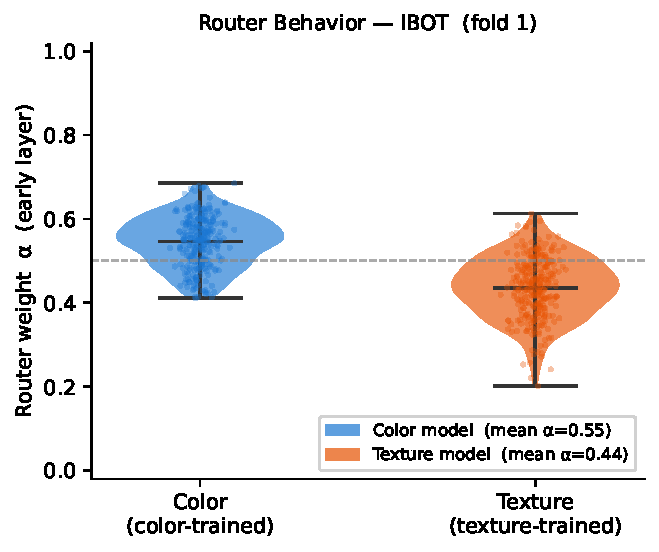
\includegraphics[width=0.46\textwidth]{fig_router_behavior.pdf}}
\caption{Distribuição dos pesos do roteador na camada rasa~$\alpha$ para
         modelos MoE treinados para cor e textura (iBOT, fold~1).
         O modelo otimizado para cor atribui consistentemente maior peso
         à camada rasa (mediana $\alpha \approx 0,55$), enquanto o modelo
         otimizado para textura desloca o peso para a camada profunda
         (mediana $\alpha \approx 0,44$, i.e., $\beta \approx 0,56$).
         Distribuições obtidas com regularização L2 no espaço de logits
         para prevenir colapso do roteamento.}
\label{fig_router}
\end{figure}

A exceção para iBOT textura~($-$1,73~pp sobre Exp.~1) é explicada pelo
fato de que o Bloco~9 do iBOT já fornece representações de textura
excepcionalmente ricas~(97,20\%); o roteador não consegue melhorar o que
já está próximo do teto do conjunto de dados.
Para VGG-16 em cor, a assimetria dimensional entre a camada rasa
pequena~(64d) e a camada profunda~(256d) pode limitar a capacidade
do projetor $h_E$.

Em termos práticos, o MoE oferece uma representação unificada para
sistemas de recuperação de atributos visuais, eliminando a necessidade
de selecionar manualmente a camada mais adequada para cada tipo de
consulta.

% -----------------------------------------------------------------------
\section{Conclusões}

Este trabalho apresentou uma avaliação abrangente da extração de
características por camada em múltiplas arquiteturas de aprendizado
profundo para classificação por cor e textura em imagens de moda, e
propôs um modelo de fusão adaptativa baseado em Mistura de
Especialistas~(MoE).

Os Experimentos~1 e~2 confirmam que o padrão de sensibilidade por camada
é consistentemente observado em todas as arquiteturas avaliadas — das
CNNs clássicas aos Transformers Visuais e Modelos de Espaço de Estados —
e que a fusão por concatenação simples não é eficaz para tarefas
específicas por atributo.
O Experimento~3 introduz o MoE como solução que aprende adaptativamente
os pesos das representações rasa~(cor) e profunda~(textura), superando
tanto a extração de camada única quanto a fusão por concatenação em 6 das
8 configurações avaliadas.
Os melhores resultados do MoE foram 98,00\%~(VMamba, textura) e
97,33\%~(iBOT, cor).

Esses achados têm implicações práticas para sistemas de recuperação de
imagens: o MoE fornece um único vetor de representação que se adapta ao
conteúdo da imagem sem requerer seleção manual de camada.
Trabalhos futuros investigarão estratégias de roteamento com mais de dois
especialistas, mecanismos de atenção entre camadas e extensão para tarefas
de recuperação em larga escala.

% -----------------------------------------------------------------------
\section*{Agradecimentos}

Este trabalho foi financiado pelo Conselho Nacional de Desenvolvimento
Científico e Tecnológico (CNPq, Brasil).

% -----------------------------------------------------------------------
\begin{thebibliography}{00}

\bibitem{b1}
S. R. Dubey, ``A decade survey of content based image retrieval using deep
learning,'' \emph{IEEE Trans. Circuits Syst. Video Technol.}, vol.~32,
no.~5, pp.~2687--2704, 2021.

\bibitem{b2}
A. Baloian, N. Murrugarra-Llerena, and J. M. Saavedra, ``Scalable visual
attribute extraction through hidden layers of a residual convnet,''
\emph{arXiv preprint arXiv:2104.00161}, 2021.

\bibitem{b3}
J. Deng, W. Dong, R. Socher, L.-J. Li, K. Li, and L. Fei-Fei,
``ImageNet: A large-scale hierarchical image database,'' in
\emph{Proc. IEEE CVPR}, 2009, pp.~248--255.

\bibitem{b4}
K. He, X. Zhang, S. Ren, and J. Sun, ``Deep residual learning for image
recognition,'' in \emph{Proc. IEEE CVPR}, 2016, pp.~770--778.

\bibitem{b7}
K. Simonyan and A. Zisserman, ``Very deep convolutional networks for
large-scale image recognition,'' \emph{arXiv preprint arXiv:1409.1556},
2014.

\bibitem{b8}
M. Moresco, A. D. S. Britto, Y. M. Costa, L. J. Senger, and
A. G. Hochuli, ``Combining multi-layer features for plant species
classification in a Siamese network,'' in \emph{Proc. IEEE SMC}, 2022,
pp.~2446--2451.

\bibitem{b10}
K. Liang, H. Chang, S. Shan, and X. Chen, ``A unified multiplicative
framework for attribute learning,'' in \emph{Proc. IEEE ICCV}, 2015,
pp.~2506--2514.

\bibitem{b11}
C. Gan, T. Yang, and B. Gong, ``Learning attributes equals multi-source
domain generalization,'' in \emph{Proc. IEEE CVPR}, 2016, pp.~87--97.

\bibitem{b12}
S. M. Youssef, ``ICTEDCT-CBIR: Integrating curvelet transform with
enhanced dominant colors extraction and texture analysis for efficient
content-based image retrieval,'' \emph{Comput. Electr. Eng.}, vol.~38,
no.~5, pp.~1358--1376, 2012.

\bibitem{b13}
A. Irtaza, M. A. Jaffar, E. Aleisa, and T. S. Choi, ``Embedding neural
networks for semantic association in content based image retrieval,''
\emph{Multimedia Tools Appl.}, vol.~72, pp.~1911--1931, 2014.

\bibitem{b15}
C. H. Lin, R. T. Chen, and Y. K. Chan, ``A smart content-based image
retrieval system based on color and texture feature,'' \emph{Image Vis.
Comput.}, vol.~27, no.~6, pp.~658--665, 2009.

\bibitem{b16}
A. Gu and T. Dao, ``Mamba: Linear-time sequence modeling with selective
state spaces,'' \emph{arXiv preprint arXiv:2312.00752}, 2023.

\bibitem{b17}
J. Zhou et al., ``iBOT: Image BERT pre-training with online tokenizer,''
\emph{arXiv preprint arXiv:2111.07832}, 2021.

\bibitem{b23}
D. Mukherjee, R. Mondal, P. K. Singh, R. Sarkar, and D. Bhattacharjee,
``EnsembleNet: A hybrid approach for vehicle detection and traffic density
estimation based on Faster R-CNN and YOLO,'' \emph{Neural Comput. Appl.},
vol.~32, no.~15, pp.~14207--14228, 2020.

\bibitem{b24}
J. Yue, Z. Li, L. Liu, and Z. Fu, ``Content-based image retrieval using
color and texture,'' in \emph{Proc. ICIG}, 2011, pp.~833--837.

\bibitem{b25}
E. Prakasa, ``Texture feature extraction by using local binary pattern,''
\emph{INKOM J.}, vol.~1, no.~1, pp.~1--6, 2016.

\bibitem{b26}
J. Long, E. Shelhamer, and T. Darrell, ``Fully convolutional networks for
semantic segmentation,'' in \emph{Proc. IEEE CVPR}, 2015, pp.~3431--3440.

\bibitem{b27}
Y. Guo, Y. Liu, T. Georgiou, and M. S. Lew, ``A review of semantic
segmentation using deep neural networks,'' \emph{Int. J. Multimedia Inf.
Retr.}, vol.~7, no.~2, pp.~87--93, 2018.

\bibitem{b28}
J. de Matos, L. E. S. de Oliveira, A. D. S. Britto Jr., and
A. L. Koerich, ``Large-margin representation learning for texture
classification,'' \emph{Pattern Recognit. Lett.}, vol.~170, pp.~39--47,
2023.

\bibitem{bzeiler}
M. D. Zeiler and R. Fergus, ``Visualizing and understanding convolutional
networks,'' in \emph{Proc. ECCV}, 2014, pp.~818--833.

\bibitem{bkazami}
H. Kazami, N. Touvron, M. Cord, and P. Perez, ``What do vision
transformers learn? A visual exploration,''
\emph{arXiv preprint arXiv:2212.06727}, 2022.

\bibitem{bmoe_orig}
R. A. Jacobs, M. I. Jordan, S. J. Nowlan, and G. E. Hinton,
``Adaptive mixtures of local experts,''
\emph{Neural Computation}, vol.~3, no.~1, pp.~79--87, 1991.

\bibitem{bmoe_cao}
Z. Cao et al., ``Multi-modal gated mixture of local-to-global experts for
dynamic image fusion,'' in \emph{Proc. IEEE/CVF ICCV}, 2023,
pp.~23555--23564.

\end{thebibliography}

\end{document}
